\documentclass[11pt]{article}
\usepackage{fullpage} %[cm]
\usepackage{lmodern} % enhanced version of computer modern
\usepackage[T1]{fontenc} % for hyphenated characters
\usepackage{amsmath}
\usepackage{amssymb}
\usepackage{microtype}
\usepackage{enumerate}
\usepackage{float}
\usepackage{ctable} % provides toprule, bottomrule, midrule
\usepackage{algorithm}
\usepackage{algpseudocode}
\usepackage{algorithmicx}
%\usepackage[ruled,linesnumbered]{algorithm2e}
\usepackage{amsthm}
\usepackage{graphicx}
\usepackage{subfig}
\DeclareCaptionType{copyrightbox}
\usepackage{color}
\newcommand{\expect}{\mathrm{Exp}}
\newcommand{\hide}[1]{}
\newtheorem{theorem}{Theorem} % {\bfseries}{\itshape}
\newtheorem{lemma}{Lemma}{\bfseries}{\itshape}
%\newdef{claim}{Claim}
%
%\theoremstyle{definition}
%\newtheorem{definition}[lemma]{Definition} % {\bfseries}{\itshape}
%
%\theoremstyle{remark}
\newtheorem{claim}[lemma]{Claim} % {\bfseries}{\itshape}
\newtheorem{observation}[lemma]{Observation} % {\bfseries}{\itshape}
%
\DeclareMathOperator*{\argmin}{arg\,min}
\newcommand{\opt}{\mathrm{OPT}}
\newcommand{\eopt}{E_{\mathrm{OPT}}}
\newcommand{\edeg}{e_{\mathrm{deg}}}
\newcommand{\prob}{\textsc{ACI}}
\newcommand{\degr}{\mathrm{d}}
\newcommand{\Vol}{\mathrm{Vol}}
\newcommand{\wmax}{w_{\max}}
\newcommand{\eps}{\epsilon}
\newcommand{\diff}{\textsc{diff}}
\newcommand{\U}{\mathcal{U}}
\newcommand{\C}{\mathcal{C}}
\newcommand{\Cw}{\mathcal{C}_w}
\newcommand{\Cwp}{\mathcal{C}_{w'}}
\newcommand{\TC}{\mathcal{T}_{\C}}
\newcommand{\commC}{\texttt{common}(\mathcal{C})}
\newcommand{\diffC}{\texttt{diff}(\mathcal{C})}
\newcommand{\diffw}{\texttt{diff}(w, w')}
\newcommand{\diffcost}{\texttt{diffcost}}
\newcommand{\diffwcost}{\texttt{diffcost}(w, w')}
\newcommand{\cut}{\texttt{cut}}
\newcommand{\ceil}[1]{\left\lceil #1 \right\rceil}
\DeclareMathOperator*{\nodes}{nodes}
\DeclareMathOperator*{\walks}{walks}
\DeclareMathOperator*{\ct}{count}
\def\algo{\textsc{greedy}}
\def\util{\texttt{util}}
\def\game{\textsc{VaccSenGame}}

\title{Persistence of anti-vaccine sentiment through strategic interactions}
\author{A S M Ahsan-Ul Haque}
\date{\today}
%
\begin{document}
\maketitle
%

\section{Introduction}

Given a social network and two competing sentiments about vaccines (pro and anti), in this study, we intend to develop a model to answer the following questions:

\begin{itemize}
    \item What is the influence of anti-vaccine movements in spreading a certain disease?
    \item How can we minimize the effects of anti-vaccine movements?
    \item How can we contain the anti-vaccines sentiment so that it does not spread outside a specific cluster? 
\end{itemize}


\noindent
\textbf{Background and motivation.} The choice of the problem selection arises from the following facts:

\begin{itemize}
    \item In recent days anti-vaccine movement is gaining momentum, and with the help of social network, they are forming clusters which can propagate anti-vaccine sentiments in the network.

    \item Despite the effort and widespread coverage of MMR vaccines, there have been massive outbreaks of measles in recent months. There have been 303 cases of measles in March 2019 alone in the US and the number is highest this year since 1992~\cite{cdc_measles}. This shows that the recent anti-vaccine movements can nullify the effectiveness of the vaccination programs.
    
    \item About 75\% of the cases in 2019 are linked to outbreaks in New York~\cite{rockland_measles}. This gives rise to the question of whether anti-vaccination movement can be strategically seeded in a network to cause a disease outbreak.

\end{itemize}

From these facts we can infer the following:
\begin{enumerate}
    \item Immunization coverage does not necessarily give us an ideal estimate of how likely a disease is going to cause an outbreak.
    
    \item Not all under-vaccinated clusters have equal potential to cause a massive disease outbreak. Some of the undervaccinated clusters might have higher interaction with the outside world, causing a greater risk of outbreaks.
    
    \item it is important to identify and sort the spatial clusters according to their potential to cause an outbreak.
\end{enumerate}


\noindent
\textbf{Objectives.} The objectives of this study are:
\begin{enumerate}
    \item Modeling and simulating the social network with mixtures of various initial states and rules of spreading for both pro and anti vaccine sentiments
    
    \item Determining the effect of network structures of the vaccination sentiments
\end{enumerate}


\noindent
\textbf{Novelty.} There have been some work on modeling vaccination sentiment~\cite{SHIM2012194}, and also, there have been several applications of competing diffusion models~\cite{prakash2012winner,bharathi2007competitive}. Modeling the spread of epidemics has been done by various diffusion processes on networks, such as the SIS or SIR models~\cite{newman2003structure, grassly2008mathematical}. However, our approach differs from the existing works in:

\begin{itemize}
    
    \item Studying the effects of network structure and their relationship with the vaccination sentiment. 
    
    \item Studying the game theoretic aspects of vaccination sentiment analysis
\end{itemize}


\section{Preliminaries}

Let the undirected unweighted graph $G=(V, E)$ denote a contact network, where $V$ is the set of nodes that represent people in the network and $E$ is the set of edges where each edge represents the connection between two people. Let, $n=|V|$ be the number of nodes in the network. Let $N(i)$ denote the set of neighbors of node $i\in V$.
\\
\\
Each node $i\in V$ has state $x_i(t)\in\{0, 1\}$ at time $t$, where 0 and 1 indicate pro- and anti-vaccine sentiments respectively.
\\
\\
Let $\mathbf{x(t)}\in\{0, 1\}^n$ denote a strategy vector at time $t$. Let $N(i, \mathbf{x}, x_i)$ be the $i^{th}$ node's neighbors who are in state $x_i$. So,  $N(i, \mathbf{x}, 0)$  denote the set of neighbors of node $i$ who are pro-vaccine and $N(i, \mathbf{x}, 1)$  denote the set of neighbors of node $i$ who are anti-vaccine, given a strategy vector $\mathbf{x}$.
\\
\\
\noindent
\textbf{Herd Immunity.} If more than a certain fraction ($\gamma$) of nodes in the entire network are vaccinated, every node gets benefited. This is known as herd immunity.
\\
\\
\noindent
\textbf{Vaccine sentiment game with herd immunity benefit.}
% Let $\gamma$ be an additional parameter, which denotes the threshold for herd-immunity, i.e., if the number of nodes vaccinated nodes exceeds $\gamma n$, then every node gets benefit $\delta$. However, if the number of vaccinated nodes is less than $\gamma n$, no one gets any benefit.
% We formalize the utility functions in the following form
% \[
% \util(i, \mathbf{x})=
% \begin{cases}
% \alpha|N(i, \mathbf{x}, x_i)| - \beta|N(i, \mathbf{x}, 1-x_i)| + \delta, \mbox{ if $\sum_i x_i < (1-\gamma)n$}\\
% \alpha|N(i, \mathbf{x}, x_i)| - \beta|N(i, \mathbf{x}, 1-x_i)|, \mbox{ otherwise}\\
% \end{cases}
% \]
% \noindent
% \textbf{added by anil.}
We have parameters $\gamma, \delta, C$. $\gamma$ is the threshold for herd-immunity, i.e., if the number of nodes vaccinated nodes exceeds $\gamma n$, then every node gets benefit $\delta$. $C$ is the benefit a node gets by vaccination.
We formalize the utility functions in the following form
\[
\util(i, \mathbf{x})=
\begin{cases}
\alpha|N(i, \mathbf{x}, x_i)| - \beta|N(i, \mathbf{x}, 1-x_i)| + \delta, \mbox{ if $x_i=1$ and $\sum_i x_i < (1-\gamma)n$}\\
\alpha|N(i, \mathbf{x}, x_i)| - \beta|N(i, \mathbf{x}, 1-x_i)|, \mbox{ if $x_i=1$ and $\sum_i x_i \geq (1-\gamma)n$}\\
\alpha|N(i, \mathbf{x}, x_i)| - \beta|N(i, \mathbf{x}, 1-x_i)| + C, \mbox{ if $x_i=0$}\\
\end{cases}
\]

\noindent
\textbf{Strong Community.} We say $S\subset V$ is a \emph{strong community} if it satisfies the following property:
\\
for each node $i\in S$, $|N(i)\cap S| \geq |N(i)-S|$, and
\\
for each $i\not\in S$, we have $|N(i)\cap S| \leq |N(i)-S|$.
\\
Intuitively, it means that every node in a strong community has at least as many nodes inside the strong community as outside.
\\
\\
\noindent
\textbf{Maximal Strong Community.} $S$ is a maximal strong community if: for each $v$, $deg_S(v)\geq deg_{V-S}(v)$
\\
We say $S\subset V$ is a \emph{Maximal Strong Community} if and only if it satisfies the following property:
\\
for each node $i\in S$, $|N(i)\cap S| \geq |N(i)-S|$, and
\\
for each $i\not\in S$, we have $|N(i)\cap S| < |N(i)-S|$.
\\
\\
\noindent
\textbf{Nash equilibrium (NE).}
We say $\mathbf{x}$ is a NE if no node $i$ is able to improve its utility by switching its state.



\begin{table}[H]
\centering
\caption{Summary of Notations}
\label{table:notations}
\begingroup
\setlength{\tabcolsep}{4pt}
\renewcommand{\arraystretch}{1.35}
\begin{tabular}{|c|l|}
\hline
Symbol          & Description                                 \\ \hline
$V$             & Set of vertices \\ \hline
$E$             & Set of edges\\ \hline
$n$   & = $|V|$, Number of nodes \\ \hline
$N(i)$       & Set of neighbors of node $i$ \\ \hline
$x_i(t)$       & State of node i at time $t$, either 0 (Pro-vaccine) or 1 (Anti-vaccine) \\ \hline
$\mathbf{x}(t)$     & Strategy vector at time $t$\\ \hline
$N(i, \mathbf{x}, x_i)$     & Set of neighbors of node i at time with state $x_i$\\ \hline
$\gamma$ & Herd immunity parameter, if $\sum_i x_i < (1- \gamma) n$ then Herd immunity exists\\ \hline
$\delta$         & Herd immunity benefit\\ \hline
$\alpha$         & Similarity benefit parameter\\ \hline
$\beta$   & Dissimilarity loss parameter\\ \hline
$C$      & Vaccination utility parameter\\ \hline
$N_s(i, \mathbf{x}, x_i)$      & Set of Node $i$'s neighbors in set s who are in state $x_i$\\ \hline
\end{tabular}
\endgroup
\end{table}
\section{The vaccine sentiment game}

% Questions to explore
% \begin{itemize}
% \item 
% When is a vector $\mathbf{x}$ a NE? 
% \begin{itemize}
%     \item When $\alpha=\beta=1$, for every strong community $S$, the state vector $\mathbf{x}$ with $x_i=0$ for $i\in S$ is a NE
%     \item 
%     What are the conditions for more general $\alpha, \beta$?
% \end{itemize}
% \end{itemize}


% \noindent
% \textbf{Vaccine sentiment game.}
We assume that people generally tend to be in the same state as most of their neighbors. So, the utility for node $i$ is defined as a linear combination of number of similar state nodes in $N(i)$ and  number of different state nodes in $N(i)$).
\\
\\
Formally, given two parameters $\alpha, \beta \in \mathbb{R}$ and $\alpha, \beta \geq  1$ , we define utility for a node $i$ in the following manner:
\begin{equation}
\label{eq:util_normal}
\util(i, \mathbf{x})=\alpha|N(i, \mathbf{x}, x_i)| - \beta|N(i, \mathbf{x}, 1-x_i)|
\end{equation}

\textbf{Rule.} A node $i$ will switch its state from $x_i$ to $(1-x_i)$ if and only if its utility gets better by switching.

\begin{align}
    x_i(t+1) &= 1-x(t)\\
    \Longleftrightarrow \util(i, \mathbf{x(t)}, 1-x_i) &> \util(i, \mathbf{x(t)}, x_i)
\end{align}
\\
\\
Otherwise, node $i$ will stay in the same state $x_i$.
\begin{align}
    x_i(t+1) &= x(t)\\
    \Longleftrightarrow \util(i, \mathbf{x(t)}, x_i) & \geq \util(i, \mathbf{x(t)}, 1-x_i)
\end{align}

\endinput

\section{Structure of Nash Equilibria}

\begin{lemma}
\label{lemma:alpha_beta_independence}
Whether or not a node will switch its state is independent of the parameters $\alpha$ and $\beta$, when C=0.

\begin{proof}
From definition, we find that,
$$N(i, \mathbf{x}, 1-x_i) = N(i) - N(i, \mathbf{x}, x_i)$$
or, $$|N(i, \mathbf{x}, 1-x_i)| = |N(i) - N(i, \mathbf{x}, x_i)|$$
or, 
\begin{equation}
\label{eq:state_subtract}
|N(i, \mathbf{x}, 1-x_i)| = |N(i)| - |N(i, \mathbf{x}, x_i)|
\end{equation}

Combining Eqn.~\ref{eq:util_normal} and Eqn.~\ref{eq:state_subtract}, we get,
$$
\util(i, \mathbf{x})=\alpha|N(i, \mathbf{x}, x_i)| - \beta (|N(i)| - |N(i, \mathbf{x}, x_i)|)
$$
or,
\begin{equation}
\label{eq:util_single_param}
\util(i, \mathbf{x})= (\alpha + \beta) |N(i, \mathbf{x}, x_i)| - \beta |N(i)|
\end{equation}\\
Now, suppose, node $i$ will switch its state after time $t$.
From the \textbf{Rule} of the game, we have,
$$x_i(t+1) = 1-x(t)$$
$$\Longleftrightarrow \util(i, \mathbf{x(t)}, 1-x_i) > \util(i, \mathbf{x(t)}, x_i)$$\\
From, Eqn.~\ref{eq:util_single_param}, we have,

\begin{align}
    \Longleftrightarrow (\alpha + \beta) |N(i, \mathbf{x}, 1-x_i)| - \beta |N(i)| &> (\alpha + \beta) |N(i, \mathbf{x}, x_i)| - \beta |N(i)|\\
    \Longleftrightarrow |N(i, \mathbf{x}, 1-x_i)| &>  |N(i, \mathbf{x}, x_i)|
\label{eq:switch_condition}
\end{align}

Similarly, node $i$ will stay in the same state $x_i$.
$$x_i(t+1) = x(t)$$
$$\Longleftrightarrow \util(i, \mathbf{x(t)}, x_i) \geq \util(i, \mathbf{x(t)}, 1-x_i)$$

From, Eqn.~\ref{eq:util_single_param}, we have,

\begin{align}
    \Longleftrightarrow (\alpha + \beta) |N(i, \mathbf{x}, x_i)| - \beta |N(i)| & \geq (\alpha + \beta) |N(i, \mathbf{x}, 1-x_i)| - \beta |N(i)|\\
    \Longleftrightarrow |N(i, \mathbf{x}, 1-x_i)| & \geq  |N(i, \mathbf{x}, x_i)|
\label{eq:stay_condition}
\end{align}

Eqn.~\ref{eq:switch_condition} and  Eqn.~\ref{eq:stay_condition} are independent of  $\alpha$ and $\beta$, which completes the proof.
\end{proof}
\end{lemma}





\begin{lemma}
For every maximal strong community $S$, the state vector $\mathbf{x}$ with $x_v=1$ for all $v\in S$ and with $x_v=0$ for all $v\notin S$ is a NE.

\begin{proof}
We will use proof by contradiction.

Suppose, there is a node $A$, which belongs to a maximal strong community S and the state vector is $\mathbf{x}$ where $x_v = 1, \forall{v \in S}$.


By this assumption, $x_A = 1$.

\begin{figure}[H]
    \centering
    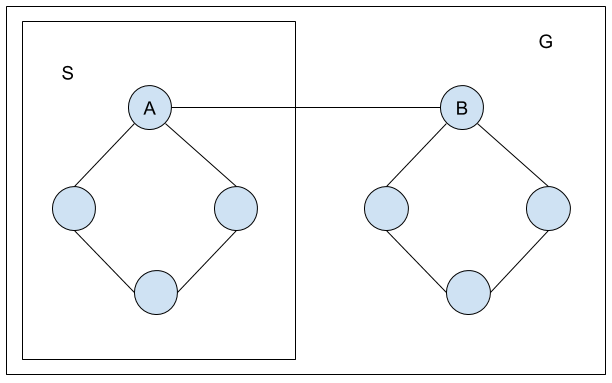
\includegraphics[width=10cm]{figs/strong_community.png}
    \caption{A Strong Community S within Graph G}
    \label{fig:strong_community}
\end{figure}

% Now, From the utility function, we can see that $A$ will switch its state if 
% \begin{align}
% \util(A, \mathbf{x}) & < 0 \\
% or, \alpha|N(A, \mathbf{x}, x_A)|  &- \beta|N(A, \mathbf{x}, 1-x_A)|  < 0 \\
% or, \alpha|N(A, \mathbf{x}, 1)|  &< \beta|N(A, \mathbf{x},0)|
% \end{align}

Now, from Lemma~\ref{lemma:alpha_beta_independence}, we have, $A$ will switch its state iff
\begin{align}
\label{eq:switch_A}
|N(A, \mathbf{x}, 1)|  < |N(A, \mathbf{x},0)|
\end{align}
\\
Now, $x_v=1, \forall{v \in S} $, which means that $x_v=1, \forall{v \in N(A) \cap S} $ \\
So, 
\begin{equation}
|N(A, \mathbf{x}, 1)| \geq |N(A) \cap S|
\end{equation}
\\
\textbf{Def.} Now, let's define $N_s(i, \mathbf{x}, x_i)$ to be the set of $i$'s of neighbors in strong community $S$ whose state is $x_i$.
\\
\\
\textbf{Def.} Similarly, let's define $N_{\bar{s}}(i, \mathbf{x}, x_i)$ to be the set of $i$'s of neighbors in $\bar{S} = G-S$ (i.e., outside the strong community $S$) whose state is $x_i$.


\begin{align}
|N(A, \mathbf{x},0)|  &= |N_s(A, \mathbf{x}, 0)| + |N_{\bar{s}}(A, \mathbf{x}, 0)|\\
& = 0 + |N_{\bar{s}}(A, \mathbf{x}, 0)|\\
& = |N_{\bar{s}}(A, \mathbf{x}, 0)|
\end{align}


Since, $N_{\bar{s}}(A, \mathbf{x}, 0) \leq|N(A) - S|$, from Eqn.~\ref{eq:switch_A}, we have,

\begin{align}
     |N(A) \cap S| < |N(A)- S|
\end{align}
% Assuming $\alpha = \beta$, we get,
% $$
% |N(A) \cap S| < |N(A)- S|
% $$
This means $A$ does not belong to the strong community, which is a contradiction.
\\
Thus, we have proved that there can be no node $A$ in $S$ which is better off by switching it's state.
\\
\\
Now, let $B$ be a node outside of the strong community $S$ which is better of by switching its state. 


Now, $x_v=1$ for all $v\in S$ and $x_v=0, \forall{v \notin S} $, which means that,
\
\begin{equation}
|N(B) - S| = |N(B, \mathbf{x}, 0)|
\end{equation}

And,
\begin{equation}
|N(B) \cap S| = |N(B, \mathbf{x}, 1)|
\end{equation}

And also, $x_B = 0$.

Now, from Lemma~\ref{lemma:alpha_beta_independence}, we have, $B$ will switch its state iff
\begin{align}
\label{eq:switch_B}
|N(B, \mathbf{x}, 1)|  > |N(B, \mathbf{x}, 0)|
\end{align}

Or.
\begin{equation}
|N(B) \cap S| > |N(B) - S|
\end{equation}

Which means that $B$ belongs to the strong community $S$, which is a contradiction. This proves that there can be no node $B \notin S$ which is better off by switching its state.
\\
\\
Combining these, we have proved that no node $A \in S$ will switch its state and no node $B \notin S$ will switch its state. Therefore, $\mathbf{x}$ is a Nash Equilibrium. 
\end{proof}

\end{lemma}

% \noindent
% \textbf{Remark.} From Eqn. (8) we see that Lemma 1 holds whenever 

% \begin{align}
    
% \end{align}
% \beta |N(A) \cap S| \geq \alpha |N(A)- S|
% $$

% \noindent
% \textbf{Structure when $\alpha\neq\beta$.}





\algdef{SE}[DOWHILE]{Do}{doWhile}{\algorithmicdo}[1]{\algorithmicwhile\ #1}

\begin{algorithm} [H]
\small{}
\caption{Sequential Best Response}\label{algo:seq-best-response}
\begin{algorithmic}[1]
    \Procedure{Sequential-Best-Response}{initial-strategy-vector}
\State $\mathbf{x}(0) \gets$ initial strategy vector
\State $|V| \gets$ len($\mathbf{x}$)
\State $\mathbf{x}(|V|) \gets$ Round1($\mathbf{x}(0)$)
\State $\mathbf{x}(2|V|) \gets$ Round2($\mathbf{x}(|V|)$)
\State \textbf{return} $\mathbf{x}(2|V|)$
\EndProcedure
\\
\\
\Procedure{Round1}{state-vector}

\State $\mathbf{x}(0) \gets$ state-vector
\State $|V| \gets$ len($\mathbf{x}$)
\For { $t \gets$ 0 to $|V|-1$}
    \State $\mathbf{x}(t+1) \gets \mathbf{x}(t) $
    
    \For{all $i \in V$ such that $x_i(t) ==  0$}
		\If{$util ( i, \mathbf{x}_{-i}(t), 1 )  >  util  ( i, \mathbf{x}_{-i}(t), 0 )$}
			\State $x_{i}(t+1) \gets 1 $
		\EndIf
\EndFor
\EndFor
\State \textbf{return} $\mathbf{x}(|V|)$
\EndProcedure
\\
\\
\Procedure{Round2}{state-vector}

\State $\mathbf{x}(0) \gets$ state-vector
\State $|V| \gets$ len($\mathbf{x}$)
\For { $t \gets$ 0 to $|V|-1$}
    \State $\mathbf{x}(t+1) \gets \mathbf{x}(t) $
    
    \For{all $i \in V$ such that $x_i(t) ==  1$}
		\If{$util ( i, \mathbf{x}_{-i}(t), 0 )  >  util  ( i, \mathbf{x}_{-i}(t), 1 )$}
			\State $x_{i}(t+1) \gets 0 $
		\EndIf
\EndFor
\EndFor
\State \textbf{return} $\mathbf{x}(|V|)$
\EndProcedure
\end{algorithmic}
\end{algorithm}
%%%%%%%%%%%%%%%%%%%%%%%%%%%%%%%%%%%%%%%%%%%%%





\begin{lemma}
The state vector $\mathbf{x}$ after Sequential Best Response is a Nash Equilibrium.

\begin{proof}
We will prove this by considering the following two cases.

\noindent
\textbf{Case 1:} Any node i in state 0 will not switch state after Round 2

At most |V| nodes can switch from 0 to 1.

At any iteration, if no node switches states: we reach NE.

So, at least 1 node must switch state in every iteration until NE.

|V| iterations are sufficient.

\noindent
\textbf{Case 2:}  Any node i in state 1 will not switch state after Round 2


There are 2 possibilities:

(a) Node i was in state 1 and didn’t switch in Round 1.

(b) Node i was in state 0 and switched in Round 2.


For both (a) and (b):

Number of nodes in state 0 can only decrease or remain unchanged after Round 2.

Utility cannot increase by switching.

\end{proof}
\end{lemma}


\begin{lemma}
Determining whether or not there exists a Nash Equilibrium with exactly K nodes in state 1 (anti-vaccine) is an NP-Hard problem.

\begin{proof}
We will prove this by reducing set-cover problem to this problem at hand.
\end{proof}
\end{lemma}
\section{Experimental Results}
\subsection{Datasets}

For the experiments we used the toy data and real world data, as shown in Table~\ref{table:dataset}.

\begin{table}[H]
\centering
\caption{Summary of Datasets}
\label{table:dataset}
\begingroup
\setlength{\tabcolsep}{4pt}
\renewcommand{\arraystretch}{1.35}
\begin{tabular}{|c|c|c|c|}
\hline
Graph          & n & $|E|$ & $\Delta(G)$\\ \hline
Small World Network (Newman\_watts\_strogatz\_graph) & 500 & 18025 &  1000\\ \hline
SNAP Facebook combined dataset~\cite{facebook_combine_data}  & 4039 & 88234 & 1612010\\ \hline
SNAP Twitter combined dataset~\cite{twitter_combined_data}  & 81306 & 1768149 & 13082506\\ \hline
\end{tabular}
\endgroup
\end{table}

\begin{figure}[H]
    \centering
    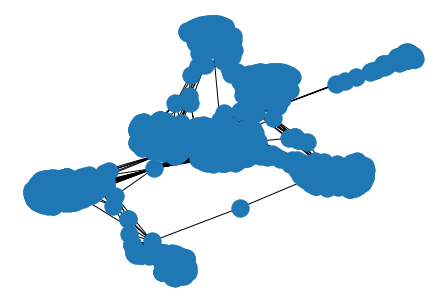
\includegraphics[width=10cm]{figs/facebook_data.png}
    \caption{SNAP (Stanford Large Network Datasets): Facebook Combined Dataset}
    \label{fig:facebook_dataset}
\end{figure}

\subsection{Hyper-parameters}
Probability of State 0 (Pro-vaccine) in initial Strategy Vector was kept at = 0.7.

\begin{table}[H]
\centering
\caption{Values of Hyper-parameters}
\label{table:hyper-params}
\begingroup
\setlength{\tabcolsep}{4pt}
\renewcommand{\arraystretch}{1.35}
\begin{tabular}{|c|l|}
\hline
Hyper-parameters          & Values\\ \hline
$\gamma$ & 0.7, 0.8, 0.9\\ \hline
$\delta$         & 0, 1, 2, 4\\ \hline
$\alpha$         & 1\\ \hline
$\beta$   & 1\\ \hline
$C$      & 1, 2, 4, 8~\cite{cvalue}\\ \hline
\end{tabular}
\endgroup
\end{table}

\subsection{Experimental Setup}
% In dataset 1, number of anti-vaccine nodes quickly diminishes to zero within <= 10 epochs.
% In dataset 2, both pro and anti vaccine sentiments co-exist in NE, within <= 20 epochs
% NE anti-vaccine fraction depends on initial x
% Usually < 0.01

% Changing $\alpha$, $\beta$ has no effect (which is evident from Lemma~\ref{lemma:alpha_beta_independence}).





\noindent
\textbf{Experiment 1:} We started with 100 different random configurations of the inital strategy vector, keeping the probability of initially being pro-vaccine fixed to 0.7. Fig.~\ref{fig:convergence_hist} shows the histogram of the time to reach the Nash Equilibrium using the SNAP dataset. As we can see from the figure, usually it takes around 3 or 4 epochs to reach the equilibrium. 

\begin{figure}[H]
    \centering
    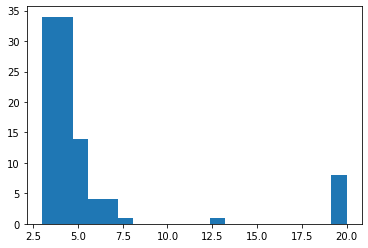
\includegraphics[width=12cm]{figs/convergence_hist.png}
    \caption{Histogram of number of epochs to reach NE}
    \label{fig:convergence_hist}
\end{figure}


Fig.~\ref{fig:exp1-diff-params} shows how the barplot changes as the hyper-parameters varry. As we can see from the figure, in this case also, in most cases, the number of epochs for convergence is less than 15.

\begin{figure}[H]
    \centering
    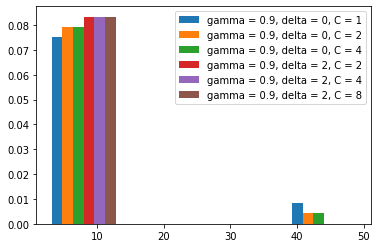
\includegraphics[width=12cm]{figs/exp1-diff-params.png}
    \caption{Histogram of number of epochs to reach NE starting with random initial strategy vector}
    \label{fig:exp1-diff-params}
\end{figure}




\begin{figure}[H]
    \centering
    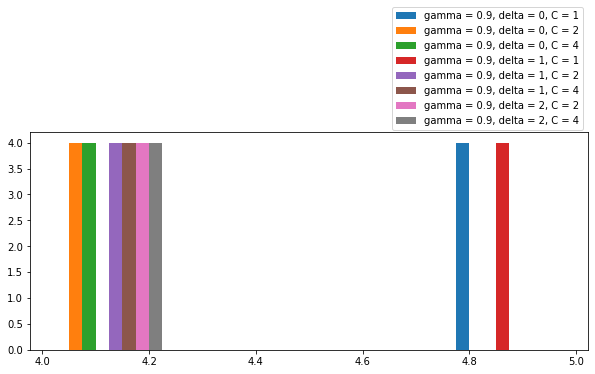
\includegraphics[width=14cm]{figs/exp1-diff-params-degree.png}
    \caption{Histogram of number of epochs to reach NE starting with highest degree nodes being anti-vaccine}
    \label{fig:exp1-diff-params-degree}
\end{figure}

\begin{figure}[H]
    \centering
    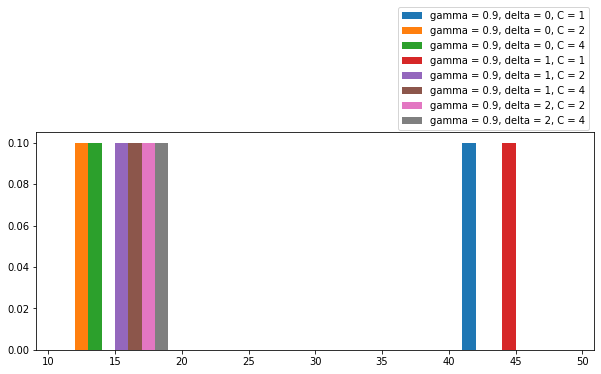
\includegraphics[width=14cm]{figs/exp1-diff-params-clusters.png}
    \caption{Histogram of number of epochs to reach NE starting nodes with highest clustering coefficients being anti-vaccine}
    \label{fig:exp1-diff-params-cluster}
\end{figure}



\noindent
\textbf{Experiment 2:} We start with the same initial strategy vector. We plot the number of unvaccinated nodes per epoch, until the network reaches an equillibrium. Fig.~\ref{fig:antivax_epoch} shows how the number of unvaccinated nodes varies with different parameters in the Facebook Combined dataset.

\begin{figure}[H]
    \centering
    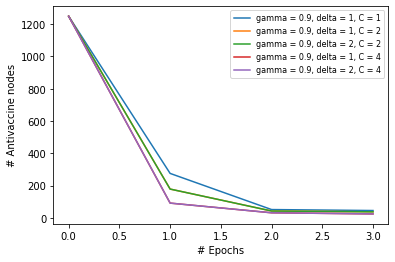
\includegraphics[width=12cm]{figs/exp1-random.png}
    \caption{Number of Antivaccine Nodes per epoch, varying the hyper-parameters}
    \label{fig:antivax_epoch}
\end{figure}


\begin{figure}[H]
    \centering
    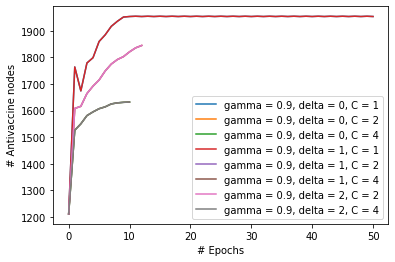
\includegraphics[width=12cm]{figs/exp2-diff-params-degree.png}
    \caption{Number of Antivaccine Nodes per epoch starting with highest degree nodes being anti-vaccine}
    \label{fig:exp2-diff-params-degree}
\end{figure}


\begin{figure}[H]
    \centering
    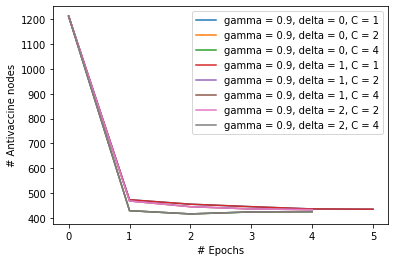
\includegraphics[width=12cm]{figs/exp2-diff-params-cluster.png}
    \caption{Number of Antivaccine Nodes per epoch, starting with nodes with highest clustering coefficient being anti-vaccine}
    \label{fig:exp2-diff-params-cluster}
\end{figure}



\noindent
\textbf{Experiment 3:} characteristics of nodes in NE: We look at the properties of nodes (e.g., degree, clustering coefficient) which end up in state 1 in experiment 2. Fig.~\ref{fig:antivax_degree} shows the histogram of the degrees of these nodes in the Facebook Combined dataset after starting with a random initial strategy vector with probability of being pro-vaccine being 0.7.

\begin{figure}[H]
    \centering
    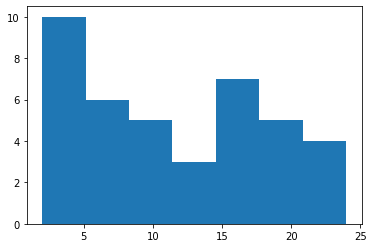
\includegraphics[width=12cm]{figs/antivax_degree.png}
    \caption{Histogram of degree of Anti-vaccine nodes in NE}
    \label{fig:antivax_degree}
\end{figure}


Fig.~\ref{fig:hist_boxplot_random}
% and~\ref{fig:boxplot_degree_cropped_1} through~\ref{fig:boxplot_degree_cropped_6} 
shows the average number of nodes having a particular degree, as well as the variance as a boxplot-- after the experiment is simulated 100 times with \textbf{random} initial strategy vectors with probability of being pro-vaccine being 0.6, $\alpha = \beta = \gamma = 1, C = 2 $ and $\delta = 0.9 $. 

\begin{figure}[H]
    \centering
    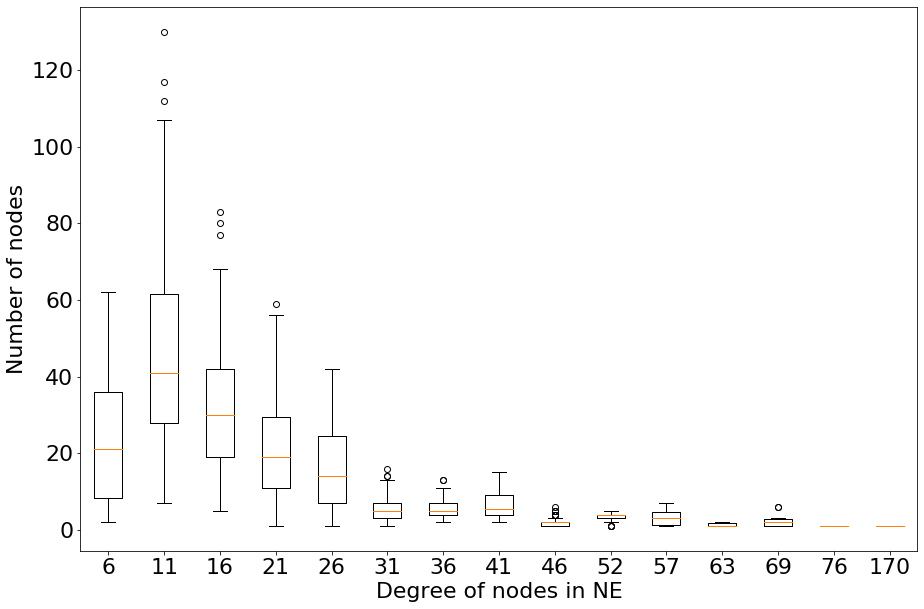
\includegraphics[width=14cm]{figs/exp3-random.png}
    \caption{Boxplot of degree of Anti-vaccine nodes in NE}
    \label{fig:hist_boxplot_random}
\end{figure}

\begin{figure}[H]
    \centering
    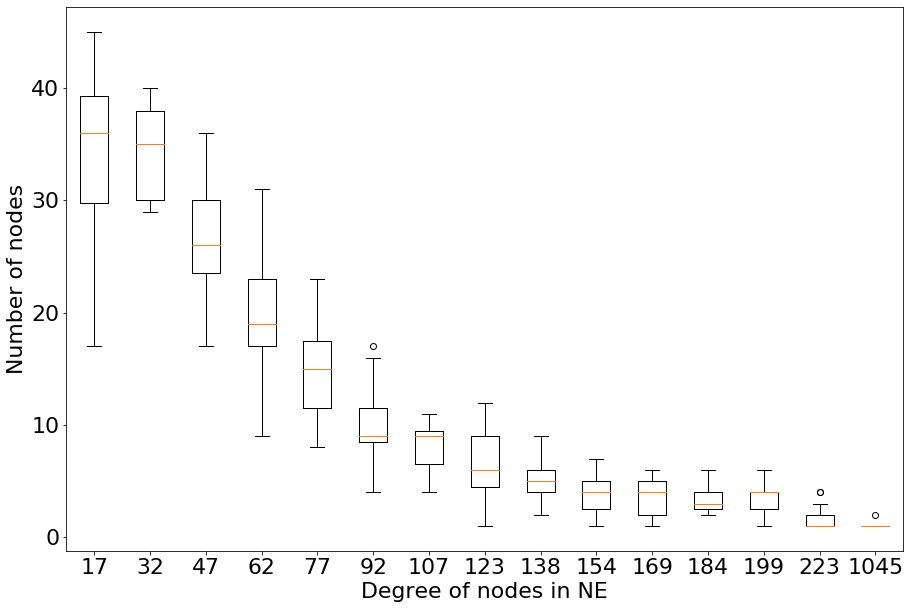
\includegraphics[width=12cm]{figs/exp3-degree.png}
    \caption{Boxplot of degree of Anti-vaccine nodes in NE, starting with highest degree nodes being anti-vaccine}
    \label{fig:exp3-degree}
\end{figure}

\begin{figure}[H]
    \centering
    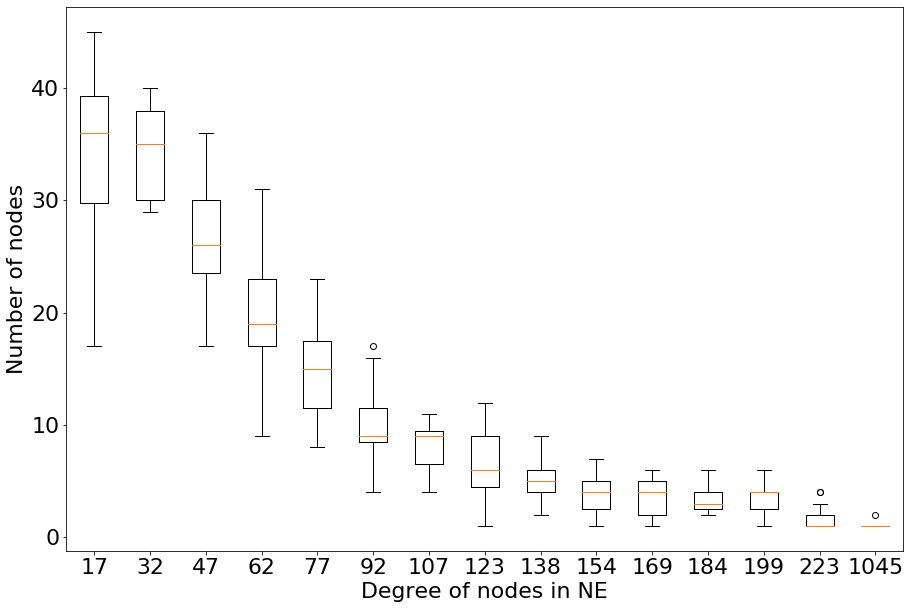
\includegraphics[width=12cm]{figs/exp3-degree.png}
    \caption{Boxplot of degree of Anti-vaccine nodes in NE, starting with nodes with highest clustering coefficient being anti-vaccine}
    \label{fig:exp3-cluster}
\end{figure}


% \begin{figure}[H]
%     \centering
%     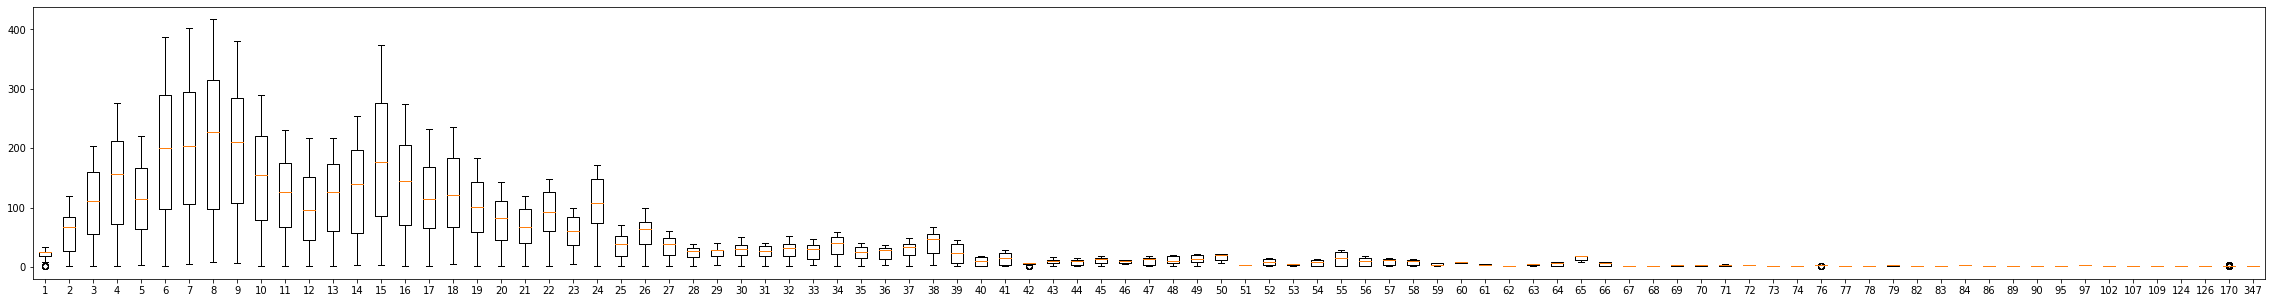
\includegraphics[width=15cm]{figs/boxplot.png}
%     \caption{Boxplot of degree of Anti-vaccine nodes in NE}
%     \label{fig:boxplot_degree}
% \end{figure}


% \begin{figure}[H]
%     \centering
%     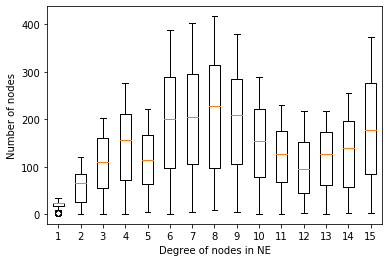
\includegraphics[width=10cm]{figs/box/1.png}
%     \caption{Boxplot of degree of Anti-vaccine nodes in NE}
%     \label{fig:boxplot_degree_cropped_1}
% \end{figure}

% \begin{figure}[H]
%     \centering
%     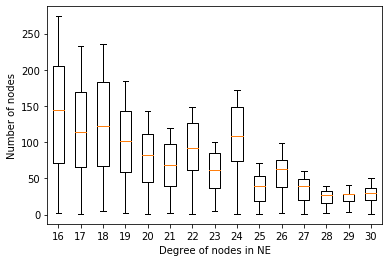
\includegraphics[width=10cm]{figs/box/2.png}
%     \caption{Boxplot of degree of Anti-vaccine nodes in NE}
%     \label{fig:boxplot_degree_cropped_2}
% \end{figure}

% \begin{figure}[H]
%     \centering
%     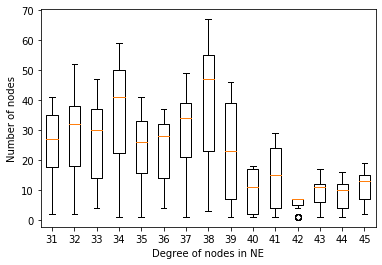
\includegraphics[width=10cm]{figs/box/3.png}
%     \caption{Boxplot of degree of Anti-vaccine nodes in NE}
%     \label{fig:boxplot_degree_cropped_3}
% \end{figure}

% \begin{figure}[H]
%     \centering
%     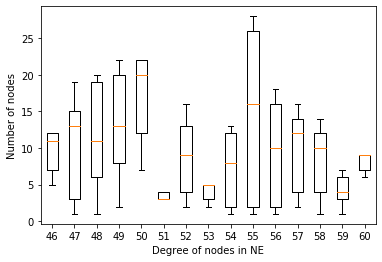
\includegraphics[width=10cm]{figs/box/4.png}
%     \caption{Boxplot of degree of Anti-vaccine nodes in NE}
%     \label{fig:boxplot_degree_cropped_4}
% \end{figure}

% \begin{figure}[H]
%     \centering
%     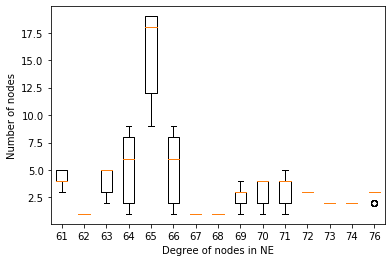
\includegraphics[width=10cm]{figs/box/5.png}
%     \caption{Boxplot of degree of Anti-vaccine nodes in NE}
%     \label{fig:boxplot_degree_cropped_5}
% \end{figure}

% \begin{figure}[H]
%     \centering
%     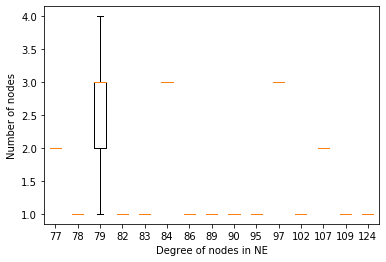
\includegraphics[width=10cm]{figs/box/6.png}
%     \caption{Boxplot of degree of Anti-vaccine nodes in NE}
%     \label{fig:boxplot_degree_cropped_6}
% \end{figure}



Fig.~\ref{fig:antivax_cluster_coeff} shows the histogram of the clustering coefficient of these nodes in the Facebook Combined dataset. As we can see, these nodes have relatively high clustering coefficients.


\begin{figure}[H]
    \centering
    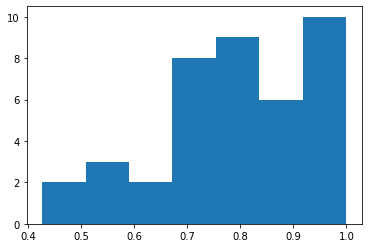
\includegraphics[width=12cm]{figs/antivax_cluster_coeff.png}
    \caption{Histogram of clustering coefficient of Anti-vaccine nodes in NE}
    \label{fig:antivax_cluster_coeff}
\end{figure}



% Experiment 4: Suppose we have some stubborn nodes S. These nodes are fixed in state 1, and their utility is not  improved by switching (this is a model). We can now see how the results in experiments 2 and 3 are affected by some stubborn nodes. There can be different strategies for picking stubborn nodes, e.g., by degree, or randomly within a community
\endinput
\section{Conclusion}

In this study, we have proposed a game theoretic model for the spreading of anti-vaccine sentiments in a network. We have discussed theoretically about the the structure of Nash Equilibrium and which factors matter most in the decision making. We have done experiments on the Small World Network and also on the Facebook Combined Dataset from Stanford Large Network Datasets (SNAP), which show the nature of the Nash Equillibrium and the nature of the anti-vaccine nodes in NE.


Some additional factors that could be included in the model in the future are:

\begin{itemize}
    \item  Some people cannot be vaccinated; they rely solely on herd immunity.
    
    \item The people in the model are not stationary, rather they can move over time and come in contact with other people from whom they can catch the disease even if their neighborhood is free from that disease. It is important to take into account such scenarios in the model.
    
    \item The price-demand relationship of vaccines is an important economic aspect of this problem. If the number of people taking the vaccines increases, the cost associated with taking the vaccines will also increase. Thus, some people will not be able to afford the vaccines.
    
\end{itemize}
\endinput

\bibliographystyle{IEEEtran}
\bibliography{ref}
\end{document}

